\documentclass[10pt,a4paper,uplatex,a4j,dvipdfmx]{jsarticle}
\usepackage[top=20truemm,bottom=15truemm,left=15truemm,right=15truemm]{geometry}
\usepackage[jis2004]{otf}
\usepackage[dvipdfmx]{graphicx}
\usepackage[dvipdfmx]{color}
\usepackage{longtable}
\usepackage{xcolor}

\usepackage{url}
\usepackage{makeidx}
\usepackage{pifont}
\usepackage{here}
\usepackage{multirow}
\usepackage{xparse}
\usepackage{xcolor}
\usepackage{listings}
\usepackage{plext}
\usepackage{footmisc}
\usepackage{amsmath}
\usepackage{amssymb}

\usepackage{multicol}


\usepackage[backend=biber,style=ieee]{biblatex}
\bibliography{report.bib}

% ソースコード
\lstset{
  basicstyle={\ttfamily},
  identifierstyle={\small},
  commentstyle={\smallitshape},
  keywordstyle={\small\bfseries},
  ndkeywordstyle={\small},
  stringstyle={\small\ttfamily},
  frame={tb},
  breaklines=true,
  columns=[l]{fullflexible},
  numbers=left,
  xrightmargin=0zw,
  xleftmargin=3zw,
  numberstyle={\scriptsize},
  stepnumber=1,
  numbersep=1zw,
  lineskip=-0.5ex
}

\usepackage{url}


\newcommand{\cmark}{\ding{51}}%
\newcommand{\xmark}{\ding{55}}%
\newcommand{\ctext}[1]{\hbox{\textcircled{\scriptsize{#1}}}}

\NewDocumentCommand{\codeword}{v}{%
    \texttt{\textcolor{black}{#1}}%
}

\renewcommand{\lstlistingname}{ソースコード}


\begin{document}

    \section*{概要}
    
    インターネット依存に対処し, 健康的な生活を送るために, インターネット利用を時間でコントロールするHTTP(S)プロキシを実装した.

    本プロキシの開発に当たり, 医療の現場で行われているインターネット依存の治療法の一つである, 「外的ストップテクニック」と呼ばれる, 一定時間が経過したらオンライン活動をストップする手法を参考にした.
    しかし現代社会において, オンライン活動をすべて遮断してしまうことは, 必要な連絡を受け取れないといった不都合を生み出してしまう. そこで, 依存しているSNSサービスなどのブロックしたいアドレスを事前に登録しておき, アクセスしてから一定時間が経過したら通信を遮断, また一定時間後に通信を再開するプロキシを実装した.
    
    実装後, LAN内にプロキシサーバを建てて運用する中で, 確かにSNS利用が抑えられ, 目の前のタスクに集中できた感触があった.
    今後は, プロキシサービスを運用し, 被験者の数を増やして行きたいと考えている. それに向けた課題も明らかとなった.

    \newpage

    \begin{multicols}{2}

    \section{目的}
    私は、SNS\footnote{Social Networking Service. WEB上にて, 社会的つながりを構築し, コミュニケーションを取るプラットフォーム. 代表的なサービスに, Facebook, Twitterなどがある.}中毒者である\footnote{河井ら \cite{kawai2011sns} のSNS依存尺度に基づく.}.
    その症状として, Twitter\footnote{米Twitter社が運営する, 短文を中心としたSNSサービス. \url{https://twitter.com}}を常に見ていないと落ち着かない\footnote{順に, 離脱症状・再燃現象・葛藤(Intrapersonal conflict) \cite{griffiths2005} \label{tw}}・Twitterを開き, 閉じようと思って閉じても気づくとTwitterを開き直している・Twitterのクライアントアプリを端末から削除しても, ブラウザからアクセスしてしまう\footref{tw}・常にTweetDeckが画面に表示されており, 作業に集中できない・Twitterをなかなか辞められないことに対する罪悪感を感じているも, 結局やめることができない\footref{tw}といったものがある.
    
    また, 世の中にはSNS中毒を含むインターネット中毒と思われる人が多数存在する.
    インターネット中毒の有病率は, イタリアの0.8\%から香港の26.7\%と調査によってばらつきがある\footnote{ばらつきがある理由として, 全世界的な調査が不足していることや, ネット中毒の定義・基準, 調査の方法論が確立していないことが挙げられる\cite{IAreview}. また, インターネットの利用環境は年々変化しており, これもばらつきの一つの要因になっていると考えられる.}ものの, 世界中で一定数の人々が発症している\cite{IAreview}.
    
  本課題では, 私を含む多くの人々がインターネット中毒に悩んでいる状況を踏まえ, 中毒状態から脱することをサポートするため, インターネット利用をコントロールするプロキシサーバを開発する.



    \section{概要}
    インターネット依存を断ち切るために, まずは利用時間の把握をすることが必要となる. 「数分だけ使うつもりだったのに, ついつい時間が経っていた」現象を防ぐため, まずは客観的にオンラインでの活動時間を記録することが効果的とされている\cite{internetaddiction}.
    モニタリングによって時間についての問題意識を獲得したら, 実際に利用時間を減らしていく必要がある. ここで有効な手段として, 「外的ストップテクニック」と呼ばれる, 一定時間にアラームが鳴ったらオンライン活動をストップするというものがある\cite{internetaddiction}. これにより, 少しづつ時間のコントロールを取り戻していくのである.

    そこで, WEBサービスにアクセスしてから一定時間後に通信を遮断し, また一定時間が経過したら通信を再開するHTTPプロキシがあれば, 時間感覚を取り戻しながら, ネットの利用頻度を減らすことができると考え, 実装した.
プログラムの名前をdetox-proxyとした.
    
    \begin{figure}[H]
      \center
      
\includegraphics[width=7cm]{img/logo.eps}
      \caption{作成したロゴ \\ スイッチの記号(JIS C 0617)をアレンジした.}
    \end{figure}

    \section{HTTP(S)プロキシの仕組み}
    
    このセクションでは, HTTP/1.1における一般的なHTTPプロキシの動作原理について, 簡単に触れておく.

    プロキシは, クライアントとサーバの通信の間に挟まり, 通信を仲介するものとして捉えるとわかりやすい.
    
    \subsection{HTTPプロキシ}
    \label{sec:http}
    まず, OSやブラウザの設定でHTTPプロキシを有効にしておく, または環境変数\codeword{HTTP_PROXY}にプロキシサーバのアドレスを指定しておく.
    こうすると, 自動的にアプリケーションのHTTP通信がプロキシを経由するようになる.
    \begin{figure}[H]
      \center
      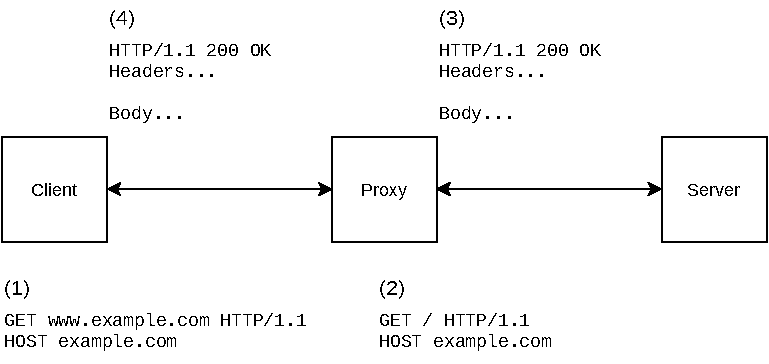
\includegraphics[width=7.5cm]{img/proxyhttp.pdf}
      \caption{HTTPプロキシの動作 \label{img:proxy:http}}
    \end{figure}
    
    図\ref{img:proxy:http}に, HTTPプロキシの動作を図解した.
    まず, クライアントがプロキシに向けて, (1)のリクエストを送る.
    ここで, メソッドの隣のパスの形式は, 通常のリクエストと違い, 絶対パスとなっている. また, \codeword{HOST}ヘッダに, リクエスト先のサーバを指定する.
    
    次に, リクエストを受け取ったプロキシは, \codeword{HOST}ヘッダに記されているアドレス宛に, (2)のリクエストを送る. ここで, 基本的にクライアントが付けたヘッダは改変せず, そのまま送信する\footnote{Forwardedヘッダ\cite{rfc:7239}など, 必要に応じてプロキシが書き換えるケースもある.}. bodyが含まれる場合は, そちらも改変せずに送信する.
    
    リクエストを受け取ったサーバは, 通常のクライアントからのアクセスと同じように\footnote{プロキシからのアクセスなのか, 通常のクライアントからのアクセスかを見極めるのは一般的に困難である.}, (3)のレスポンスを返す. レスポンスを受け取ったプロキシは, その内容をそのままクライアントへと返す(4).
    
    このような動作で, プロキシはクライアントとサーバとのやり取りを仲介するのである. (1)のリクエストを受け取った段階で, \codeword{HOST}ヘッダを見て通信を遮断するといったことや, (3)のレスポンスのヘッダやボディを見て有害なものが含まれていないかチェックするといったことが可能となる.

    \subsection{HTTPSプロキシ}
    セクション\ref{sec:http}で紹介したHTTPプロキシの仕組みは, そのままHTTPS通信に用いることができない. なぜならHTTPS通信においては, 通信が暗号化されており, ヘッダなどの中身をプロキシが見ることはできないからである\footnote{なおプロキシサーバの証明書を発行し, 通信の途中(プロキシ)で通信内容を復号し, チェックした上で再度暗号化して転送するものも存在する. 本稿では扱わない.}.
    サーバとクライアント間のエンドツーエンド暗号化を実現しつつ, プロキシサーバを機能させるために, HTTP/1.1では\codeword{CONNECT}メソッドが用意されている\cite{rfc:7231}.

    \begin{figure}[H]
      \center
      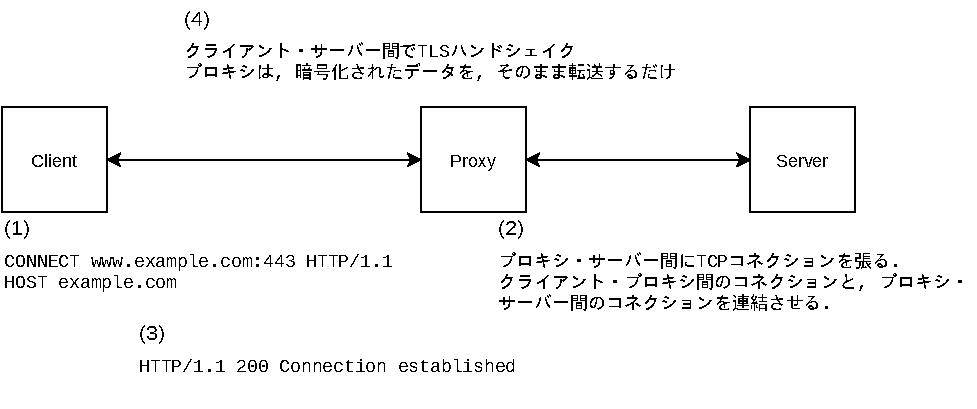
\includegraphics[width=7.5cm]{img/proxyhttps.pdf}
      \caption{HTTPSプロキシの動作 \label{img:proxy:https}}
    \end{figure}
    
    図\ref{img:proxy:https}に, \codeword{CONNECT}メソッドを用いたプロキシの動作を示した.
    まず, クライアントはプロキシに\codeword{CONNECT}メソッドを使ってリクエストを送信する.
    リクエストを受け取ったプロキシは, パスに記されているサーバのアドレス・ポートにTCPコネクションを張る. そして, これ以降クライアントから送られてきたデータは, 直接このコネクションへ流し込む. また, サーバから送られてきたデータも, そのままクライアントとのコネクションへ流す.
    これにより, 仮想的にクライアント・サーバ間に1本のコネクションが貼られたことになる(2).
    
    その後, プロキシはクライアントへ200番台のレスポンスを返す(3).
    クライアントは, これでプロキシの先にサーバへのコネクションが張られたとみなし, 通常のプロキシを介さないアクセスと同じ手順でTLSハンドシェイクを開始し, サーバとセキュアな通信を行う.

    \section{仕様と実装}
    % 全体の仕様
    \begin{figure}[H]
      \center
      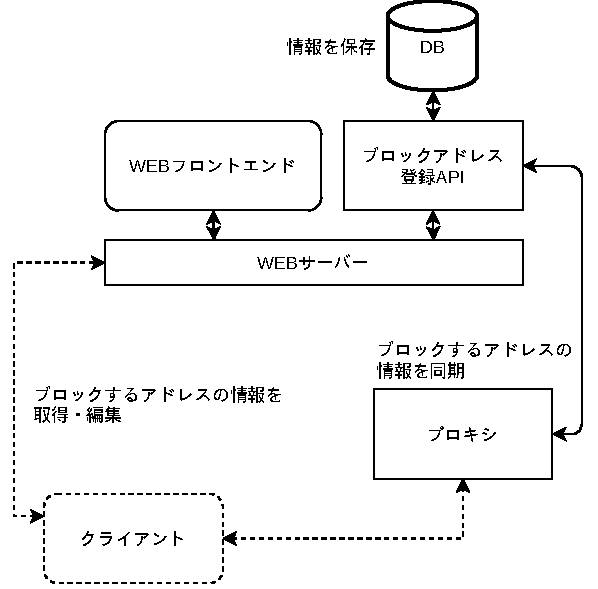
\includegraphics[width=7cm]{img/proxyall.pdf}
      \caption{detox-proxyの全体像 \label{img:proxy:all}}
    \end{figure}
    
    図\ref{img:proxy:all}に, detox-proxyの構成を示した.
    まず, ブロックするアドレス・遮断時間などを登録するデータベースと, それに対しCRUD操作を行うREST APIサーバを用意する. またWEBのフロントエンドを用意し, ユーザはフロントエンドを介してAPIにリクエストを送り, ブロックするアドレスを登録・編集できるようにする.
    プロキシは, APIから登録されたブロックアドレスを取得し, 内部のメモリに保存する. クライアントからのHTTPリクエストが来るたびに, リクエスト先のアドレスがブロックリストに登録されていないか, されている場合制限時間内のアクセスかを把握し, 通信の仲介・遮断を行う.
    
    なお, 開発を効率化するため, API・DB・WEBサーバ・プロキシはコンテナ化した.
    また, それらのコンテナをオーケストレーションツールであるdocker-composeを用いて管理し, 用意にデプロイ・起動できるようにした.
    
    以下に, フロントエンド・APIサーバ・プロキシサーバについてその仕様と, 実装を説明する.

    \subsection{フロントエンド}
    フロントエンドは, Elm\cite{elm}で実装した.
    Elmは強い静的型付けを持つ関数型のDSL
    \footnote{Domain-Specific Language. 汎用言語と異なり, 特定のタスクに特化した言語. Elmは, WEBフロントエンドの開発に特化した言語である.}
    で, Haskell\cite{haskell}に似た文法を持つ. Elmは, Javascriptに変換されるトランスパイル言語である.

    TEAアーキテクチャ\footnote{プログラムを, Model・View・Updateに分割し, それぞれにアプリケーションの状態を保持・状態をHTMLに変換・メッセージを使って状態を更新する役割を担わせる. これにより, 見通しのよいプログラムが生まれる.\cite{elm:tea}}
    に沿って, 副作用のない安全なSPA\footnote{Single Page Applicationの略.}を作ることができ, また変化の激しいフロントエンド界隈から一歩距離を置き, 穏やかに開発できることから, この言語を採用した.
    また, デザインは図\ref{img:front}のように, Neumorphism\footnote{スキューモーフィズムとフラットデザインの両方を取り入れたようなデザイン.}
    を取り入れた, 立体感のあるわかりやすいものとした.
    
    \begin{figure}[H]
      \center
      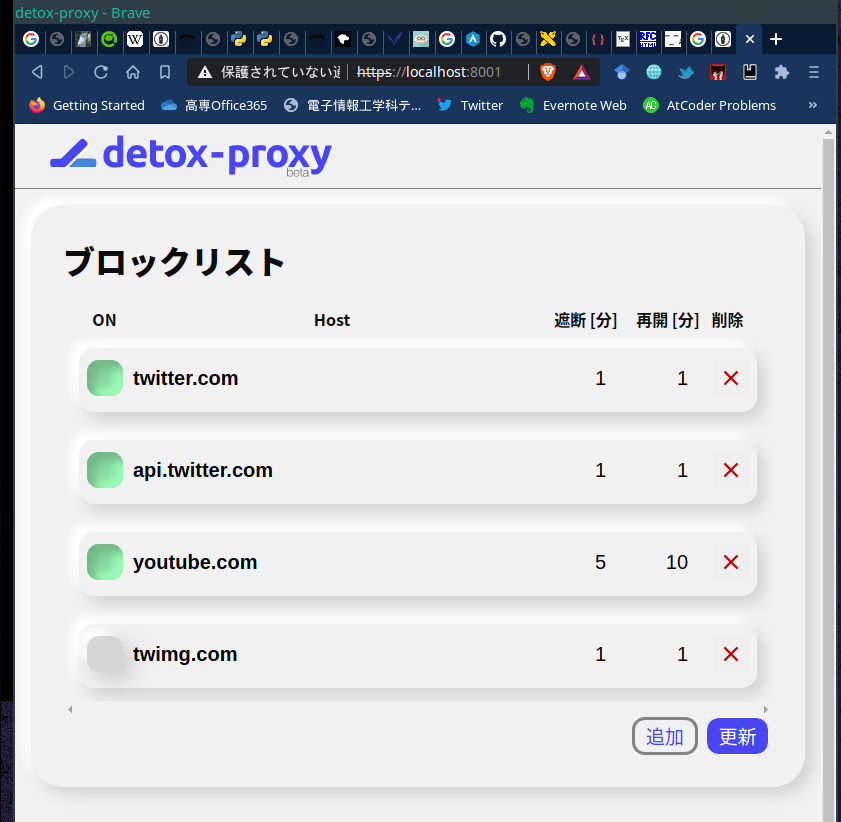
\includegraphics[width=7cm]{img/front.png}
      \caption{フロントのスクリーンショット \label{img:front}}
    \end{figure}
    

    \subsection{APIサーバ}
    
    APIサーバは, Python及びマイクロ・WEBアプリケーション・フレームワークであるFastAPI\cite{fastapi}を使用した. FastAPIは, 簡単にPythonの型ヒントに基づいて, REST APIが構築できる特徴を持つ.
    
    作成したエンドポイントは, 次の5つである.
    
       \subsubsection*{GET /api/blockaddress}
          \begin{description}
            \item[概要] ブロックアドレスのリストを取得する.
            \item[Response] \codeword{List[Block]}
          \end{description}

       \subsubsection*{POST /api/blockaddress}
         \begin{description}
            \item[概要] ブロックアドレスを新規登録する
            \item[Request] \codeword{List[BlockCreate]}
            \item[Response] \codeword{List[Block]}
          \end{description}

       \subsubsection*{PUT /api/blockaddress}
           \begin{description}
            \item[概要] 既存のブロックアドレスの情報を更新する.
            \item[Request] \codeword{List[Block]}
            \item[Response] \codeword{List[Block]}
          \end{description}

       \subsubsection*{DELETE /api/blockaddress}
           \begin{description}
            \item[概要] 登録されたブロックアドレスを削除する.
            \item[Request] \codeword{List[Int]} (Blockのidを指定)
          \end{description}

       \subsubsection*{GET /proxy.pac}
           \begin{description}
            \item[概要] PACファイル\footnote{Proxy Auto-Configuration. プロキシの設定情報を含むファイル. 内部にはJavascriptが書かれており, アクセス先に応じて使うプロキシを変更すると言った挙動も可能. \cite{moz:pac}}をダウンロードする.
            \item[Response] PACファイル.
          \end{description}
       
       なお, 上記中の\codeword{Block}・\codeword{BlockCreate}は, ソースコード\ref{jsonObject}に示す形式のJSONオブジェクトである.

       \begin{lstlisting}[caption=各JSONオブジェクト,label=jsonObject]
Block: {
  id      : integer ブロックリストのID
  url     : string  ブロックするアドレス
  start   : integer 初回アクセスからstart分経過したら遮断
  end     : integer 初回アクセスからstart + end分経過したらリセット 
  active  : boolean このブロック情報が有効かどうか
}

BlockCreate: {
  url     : string
  start   : integer
  end     : integer
  active  : boolean
}
      \end{lstlisting}

また, APIサーバの起動時に, \codeword{GET /api/blockaddress}で取得できるものと同じデータをプロキシサーバに送信し, ブロックリストの同期を図る.

  \subsection{プロキシサーバ}
    
    detox-proxyの中核となるプロキシは, Nim\cite{nim}で実装した.
    Nimは, Pythonに似た文法を持つ, 静的型付け言語である. C言語にトランスパイルされる\footnote{C言語以外にも, C++, Objective-C, Javascriptなど, いくつかの言語にトランスパイルすることができる.}ため, 高速なプログラムを実装することができるという特徴を持つ. また\codeword{async/await}構文による非同期処理が書きやすく, ネットワークプログラミングに適していると考え採用した.
    
    プロキシサーバでは, まずTCPソケットを作成し, 5001番ポートでlistenする.
    クライアントからのアクセスがあれば, HTTPリクエストをパースし, リクエストされたサーバへ新たにTCPコネクションを張る. その後, リクエストの種類に応じてセクション\ref{sec:proxy:http}及び\ref{sec:proxy:https}に記した挙動をする.
    \subsubsection{HTTPリクエスト (CONNECTメソッド以外)}
    \label{sec:proxy:http}
    クライアントから送られたデータを, サーバへ流す.
    サーバからレスポンスを受け取ったら, そのままクライアントへ送信する.
    以上の動作が終了したら, クライアント・プロキシ間, プロキシ・サーバ間それぞれのTCPコネクションを切断する.
    
    \subsubsection{HTTPSリクエスト (CONNECTメソッド)}
    \label{sec:proxy:https}
    クライアントへ, \codeword{HTTP/1.1 200 Connection Established}レスポンスを返す.
    その後, クライアント・プロキシ間及び, プロキシ・サーバ間のTCPコネクションを結合させ, 双方向にデータを転送する.
    2つのコネクションを監視し, どちらかのコネクションの切断を検知したら, 自動的にもう一方も切断する.
    
    \subsubsection{遮断処理}
    本セクションでは, 指定されたアドレスとの接続を, 遮断する処理について解説する.
    
    APIサーバの起動時に, ソースコード\ref{jsonObject}中に示した\codeword{Block}データが送られてくるので, メモリ上に保持する. また, ブロックリストに含まれるアドレスについては, アクセスログもメモリ上に保持する.

    クライアントからリクエストが来るたびに, アクセス先のアドレスがブロックリストに含まれていないかチェックし, 含まれていなければ接続する.
    含まれていた場合は, アクセスログを参照し, アクセスから\codeword{Block.start}分経過していなければ接続する. 経過していた場合は, \codeword{Block.start + Block.end}分経過しているかチェックし, 経過していれば接続し, 経過していなければ接続を遮断する(TCPコネクションを切断する).

    \section{結果}
    求めていたプロキシが実装できた.
    実際に1日使用してみたところ, Twitterの利用頻度・ツイート数が減少し, 締め切り直前のレポート執筆作業に集中することができた.
    
    \section{今後の課題と解決策}
    今後は, プロキシサービスを運用し, 多くの人に使ってもらい, このプロキシがインターネット中毒の治療に効果を発揮するのか検証していきたいと考えている.
    それに向け, 現在明らかになっている課題を以下に示す.
    
    \subsection{セキュアな接続}
    \label{sec:secure}
    現在, クライアント・プロキシ間が平文でやり取りされている.
    これは, HTTP接続だけでなく, HTTPS接続において\codeword{CONNECT}リクエストをプロキシに送信するときも同様である.
    このままでは, 通信内容を途中で第3者に把握されたり, 改ざんされる危険性がある.
    
    そこで, クライアント・プロキシ間の通信をTLS化する必要がある.
    実際に実装したが, アプリケーションによって対応がまちまち\footnote{cURL\cite{curlhttps}, Chrome\cite{chromehttps}, Firefox\cite{firefoxhttps}といったアプリケーションは対応している. その一方で, ほとんどのアプリケーションは対応の兆しを見せておらず, プロキシサーバが426を返しても無反応のまま通信が途切れてしまう.}
    で, 安定した接続ができなかったため, コードを削除した.
      
    \subsection{認証}
    \label{sec:auth}
    APIサーバにユーザ登録機能を設け, ユーザごとにブロックするアドレスを設定できるようにする必要がある.
    またプロキシにはユーザ名とパスワードによるBASIC認証機構を実装し, ユーザに応じた社団処理を行う必要がある.
    
    こちらについても実装した. しかし, アプリケーションによってBASIC認証の対応がまちまちであり, OSの設定で認証を有効化しても, ブラウザ以外の殆どのアプリケーションが\codeword{Proxy-Authorization}ヘッダを付与せず, また407レスポンスに対応しなかった. 安定して動作しなかったため, 削除した.
    
    \subsection{解決策}
    \label{sec:resolv}
    セクション\ref{sec:secure}・\ref{sec:auth}で示した課題を解決するため, TCP・UDPのプロキシを作成し, 各クライアントに作成したTUNデバイスなどからアクセスすることでこうしたアプリケーションの制約を受けないようにし, 想定通りのサービスを実現させたい.
    
    
    \section{終わりに}
    HTTPについての理解もあやふやだった自分が, 時間をかけつつも一からHTTP(S)プロキシを実装できたことに, 大変な喜びを感じている.
    長期間に渡る使用を通じて, SNS依存から脱却し, 生産的な学生生活が送れるようになることを期待している.
    
    今後は, ネットワークプログラミングについて深く学び, セクション\ref{sec:resolv}で示したTCP・UDPプロキシの実装に励みたい. 最終的にはプロキシサービスを運営し, 世界中のインターネット依存症で苦しむ人のサポートをしたい.
    \end{multicols}


  \printbibliography[title=参考文献]
  
  \section*{ソースコード}
  本課題で作成したソースコードは, \url{https://github.com/kekeho/detox-proxy}にて, MITライセンス\cite{detox:license}で提供している.
  
  \section*{備考}
  本課題の他に, 環境情報学部入学予定 後藤 大介君と一緒に, 2021年入学のSFC生が現在行っているプロジェクトを共有するページ(\url{https://projshare.com/})の実装を行った. 主にサーバサイドを担当した.
\end{document}
